%% =====================================================================
%%  MLEE Course Project Poster Template  (BITS Pilani, EEE Department)
%%  Format : A0 portrait, tikzposter class
%%  Build  : pdflatex MLEE_Poster_Template.tex   (run twice)
%%
%%  HOW TO USE
%%  1. Put the BITS logo in this folder as  bits_logo.png  (or .pdf/.jpg
%%     and edit \biTSlogofile below). The dashed placeholder is replaced
%%     automatically once the file exists.
%%  2. Edit title, authors, instructor, team ID in the preamble.
%%  3. Replace the guideline text in every block with your own content.
%%  4. Replace each figure placeholder: save your plots as fig_method.png,
%%     fig_result1.png, fig_result2.png (or change the names in \figslot).
%%  5. Delete the "Poster Guidelines" block before printing.
%%
%%  The poster and the written report are complementary and equally
%%  weighted. Keep title, numbers, terminology and key figures identical.
%% =====================================================================
\documentclass[30pt, a0paper, portrait, margin=0mm, innermargin=15mm,
               blockverticalspace=15mm, colspace=15mm, subcolspace=8mm]{tikzposter}

\usepackage[T1]{fontenc}
\usepackage[scaled]{helvet}
\renewcommand{\familydefault}{\sfdefault}
\usepackage{amsmath, amssymb}
\usepackage{booktabs}
\usepackage{enumitem}
\usepackage{graphicx}

% ---------------------------------------------------------------------
%  FILE NAMES  (edit these if your files are named differently)
% ---------------------------------------------------------------------
\newcommand{\bitslogofile}{bits_logo.png}      % BITS Pilani logo
\newcommand{\sidelogofile}{dept_logo.jpg}      % optional: department / lab logo
\newcommand{\qrfile}{qr_code.png}              % optional: QR to report / code

% ---------------------------------------------------------------------
%  COLOURS  (BITS-style navy and blue)
% ---------------------------------------------------------------------
\definecolor{bitsnavy}{HTML}{1F3864}
\definecolor{bitsblue}{HTML}{2E75B6}
\definecolor{bitsgold}{HTML}{C9A227}
\definecolor{guidegrey}{HTML}{5F5F5F}

\definecolorstyle{BITSStyle}{
  \colorlet{colorOne}{bitsnavy}
  \colorlet{colorTwo}{bitsblue}
  \colorlet{colorThree}{bitsgold}
}{
  \colorlet{backgroundcolor}{white}
  \colorlet{framecolor}{bitsnavy}
  \colorlet{titlefgcolor}{white}
  \colorlet{titlebgcolor}{bitsnavy}
  \colorlet{blocktitlebgcolor}{bitsblue}
  \colorlet{blocktitlefgcolor}{white}
  \colorlet{blockbodybgcolor}{white}
  \colorlet{blockbodyfgcolor}{black}
  \colorlet{innerblocktitlebgcolor}{bitsblue}
  \colorlet{innerblocktitlefgcolor}{white}
  \colorlet{innerblockbodybgcolor}{white}
  \colorlet{innerblockbodyfgcolor}{black}
  \colorlet{notefgcolor}{black}
  \colorlet{notebgcolor}{bitsblue!10}
  \colorlet{noteframecolor}{bitsblue}
}
\usecolorstyle{BITSStyle}
\usetitlestyle[width=0.97\textwidth]{Default}
\useblockstyle{Default}
\usebackgroundstyle{Default}

% ---------------------------------------------------------------------
%  HELPER MACROS
% ---------------------------------------------------------------------
% Logo slot: real logo if the file exists, else a dashed placeholder.
% #1 = file, #2 = placeholder text
\newcommand{\logoslot}[2]{%
  \IfFileExists{#1}{%
    \includegraphics[height=7cm, width=\linewidth, keepaspectratio]{#1}%
  }{%
    \begin{tikzpicture}
      \node[draw=white, dashed, line width=2pt, minimum width=10cm,
            minimum height=7cm, text=white, align=center,
            font=\Large\itshape] {#2};
    \end{tikzpicture}%
  }%
}

% Figure slot: real figure if the file exists, else a dashed placeholder.
% #1 = file, #2 = width, #3 = height, #4 = placeholder text
\newcommand{\figslot}[4]{%
  \begin{center}
  \IfFileExists{#1}{%
    \includegraphics[width=#2, height=#3, keepaspectratio]{#1}%
  }{%
    \begin{tikzpicture}
      \node[draw=guidegrey, dashed, line width=2pt, minimum width=#2,
            minimum height=#3, text=guidegrey, align=center,
            font=\Large\itshape, text width=\dimexpr#2-2cm\relax] {#4};
    \end{tikzpicture}%
  }%
  \end{center}%
}

% Figure / table caption
\newcommand{\figcap}[1]{{\par\centering\small\itshape #1\par}\vspace{4mm}}

% Grey italic guideline text (replace with your own content)
\newcommand{\guide}[1]{{\color{guidegrey}\itshape\small Guideline: #1\par}\vspace{3mm}}

% Compact lists
\setlist[itemize]{leftmargin=1.2em, itemsep=2pt, topsep=2pt, parsep=0pt}
\setlist[enumerate]{leftmargin=1.5em, itemsep=2pt, topsep=2pt, parsep=0pt}

% ---------------------------------------------------------------------
%  TITLE, TEAM, AFFILIATION  (edit)
% ---------------------------------------------------------------------
\title{Hand-Drawn Circuit Schematics to LTspice Netlists}
\author{[Student Name 1] \;\textbullet\; [Student Name 2] \;\textbullet\; [Student Name 3]
        \;\;|\;\; Team [ID]}
\institute{Department of Electrical and Electronics Engineering, BITS Pilani, Pilani Campus
           \;\textbullet\; MLEE \;\textbullet\; Instructor: [Name] \;\textbullet\; Semester I, 2026--27}

\makeatletter
\settitle{%
  \centering
  \begin{minipage}[c]{0.16\linewidth}\centering
    \logoslot{\bitslogofile}{[ BITS Pilani\\logo here ]}
  \end{minipage}%
  \begin{minipage}[c]{0.64\linewidth}\centering\color{titlefgcolor}
    {\bfseries\fontsize{54}{64}\selectfont \@title \par}
    \vspace{1.2em}
    {\fontsize{36}{44}\selectfont \@author \par}
    \vspace{0.6em}
    {\fontsize{28}{34}\selectfont \@institute \par}
  \end{minipage}%
}
\makeatother

\begin{document}
\maketitle

% =====================================================================
\begin{columns}
% ------------------------- LEFT COLUMN -------------------------------
\column{0.5}

\block{Summary}{
  Turning a hand-drawn circuit into a simulation is still done by hand. Prior
  work recognises \emph{components} well---94--96\%---but stops before a usable
  circuit, and the one published attempt at simulation was limited to purely
  parallel circuits. We build the full chain from photograph to a
  \textbf{working LTspice schematic}, and score it by graph isomorphism against
  reference netlists. Components are recovered at \textbf{F1 0.966}; the
  exactly correct circuit at only \textbf{0.333}. \textbf{Finding the parts
  is solved; wiring them up is not.}
}

\block{Introduction and Objectives}{
  \textbf{Motivation:} engineers sketch circuits on paper long before they draw
  them in software. Retyping every component and connection into a schematic
  editor is slow and error-prone; a photograph should be enough.
  \vspace{3mm}

  \textbf{Objectives:}
  \begin{itemize}
    \item Train a symbol detector on CGHD---the labelled bounding-box dataset
          prior work said \textit{``was not to be found on the web''}.
    \item Recover connectivity for \textbf{arbitrary} topologies, not just the
          parallel circuits prior work was restricted to.
    \item Evaluate the output \textbf{as a circuit}, by graph isomorphism
          against reference schematics---not as a set of labels.
  \end{itemize}
}

\block{Background}{
  \textbf{Key idea:} a circuit is a labelled bipartite graph of components and
  electrical nodes. Two extractions describe the same circuit when their graphs
  are isomorphic under a type-preserving map:
  \[ G=(C \cup N,\;E), \qquad
     \hat{G} \cong G^{*} \iff \exists\,\phi:\; \text{type}(\phi(c))=\text{type}(c) \]
  \begin{itemize}
    \item MobileNet on isolated crops reaches 96\%, but grid and sliding-window
          scanning of full schematics \textit{``performed poorly''} [1]
    \item A CNN plus sliding windows reaches 79.4\% box accuracy and emits a
          netlist \textbf{for parallel circuits only}---general node detection
          \textit{``proved to be a daunting task''} [2]
    \item \textbf{Gap:} nobody evaluates whether the \emph{recovered circuit} is
          correct. We do, using CGHD's reference schematics [4].
  \end{itemize}
}

\block{Methodology}{
  \figslot{fig_method.png}{0.93\linewidth}{13cm}%
    {Figure placeholder\\Pipeline / block diagram of the approach\\(save as fig\_method.png)}
  \figcap{Figure 1: Detected symbols are \emph{erased} from the binarised image;
  what remains is wires. Their skeleton is labelled into electrical nodes.}
  \begin{enumerate}
    \item \textbf{Data:} CGHD [4], 3{,}269 photographs, 248k boxes, 59 labels
          merged to 16; split \textbf{by drafter}, never by image.
    \item \textbf{Detect:} YOLOv8s @ 896\,px, 50 epochs.
    \item \textbf{Clean:} flat-field division + Otsu, then a
          \textbf{stroke-thickness filter} to strip printed page ruling.
    \item \textbf{Trace:} skeleton $\rightarrow$ connected components
          $\rightarrow$ nodes; junctions union, crossovers re-link collinear stubs.
    \item \textbf{Write:} SPICE deck + LTspice \texttt{.asc}.
  \end{enumerate}
}

\block{Experimental Setup}{
  \begin{center}
  \begin{tabular}{ll}
    \toprule
    \textbf{Parameter} & \textbf{Value / description} \\
    \midrule
    Dataset        & CGHD, 3{,}269 photographs, 16 merged classes \\
    Split          & by drafter: 4 test, 3 validation \\
    Detector       & YOLOv8s, 896\,px, 50 epochs, mosaic + flips \\
    Evaluation     & 96 photographs with reference LTspice schematics \\
    Tools          & PyTorch, Ultralytics, OpenCV, NetworkX, LTspice 26.1.1 \\
    \bottomrule
  \end{tabular}
  \end{center}
}


% ------------------------- RIGHT COLUMN ------------------------------
\column{0.5}

\block{Results}{
  \figslot{fig_result2.png}{0.93\linewidth}{8cm}%
    {Figure placeholder\\Per-stage results\\(save as fig\_result2.png)}
  \figcap{Figure 2: The gap between finding the parts (0.966) and recovering
  the circuit (0.333) \emph{is} the finding.}

  \begin{center}
  \begin{tabular}{lll}
    \toprule
    \textbf{Method} & \textbf{Task} & \textbf{Score} \\
    \midrule
    HOG+SVM [3], reimplemented & isolated crops   & 0.920 \\
    Reported in [1] / [2]      & isolated crops   & 0.960 / 0.954 \\
    \midrule
    YOLOv8s detector & mAP@50 (val drafters) & 0.807 \\
    \midrule
    This work & bill of materials (F1) & 0.966 \\
    This work & local topology (F1)    & 0.453 \\
    \textbf{This work} & \textbf{whole circuit (exact)} & \textbf{0.333} \\
    \bottomrule
  \end{tabular}
  \end{center}
  \figcap{Table 1: Scored by graph isomorphism against reference netlists.}

  \figslot{fig_result3.png}{0.93\linewidth}{7cm}%
    {Figure placeholder\\Ground-truth boxes vs trained detector\\(save as fig\_result3.png)}
  \figcap{Figure 3: Swapping perfect boxes for the trained detector costs about
  one point of exact match. \textbf{The detector is not the bottleneck.}}

}

\block{Discussion}{
  \begin{itemize}
    \item \textbf{Finding:} mid-nineties accuracy on isolated crops is real but
          measures a \emph{sub-problem}. Asked to produce a circuit, performance
          is governed by connectivity, which no reference work evaluates.
    \item \textbf{Why ruling matters:} adaptive thresholding equalises local
          contrast, promoting a faint printed rule line to the status of a
          pencil stroke. One such line spans the page and welds every node into
          one. Removing it \emph{by component} fails---where it crosses a wire
          the two are one component. \textbf{Thickness cuts the crossing
          instead:} ruling is 1--2\,px, pencil 3--6\,px.
    \item \textbf{Strength:} every schematic passing verification opens and
          simulates in LTspice; arbitrary topologies, not parallel only.
    \item \textbf{Limitation:} values are not read (defaults, user-editable);
          3-terminal pin order is positional; evaluation uses one drafter's
          96 photographs---the only ones with reference schematics.
  \end{itemize}
  \vspace{2mm}
  \begin{center}
  \begin{tabular}{lcc}
    \toprule
    \textbf{Pre-processing} & \textbf{Exact} & \textbf{Local F1} \\
    \midrule
    CLAHE + adaptive threshold \textit{(prior work)} & 0.250 & 0.328 \\
    Flat-field division + Otsu                       & 0.281 & 0.402 \\
    \textbf{+ stroke-thickness filter}               & \textbf{0.333} & \textbf{0.453} \\
    \bottomrule
  \end{tabular}
  \end{center}
  \figcap{Table 2: Printed page ruling, not symbol recognition, dominates the error.}
}

\block{Conclusion and Future Work}{
  \begin{itemize}
    \item Complete photograph $\rightarrow$ LTspice path; components at
          \textbf{F1 0.966}, exact circuit at \textbf{0.333}.
    \item Component recognition is largely solved; \textbf{connectivity recovery
          is the open problem}.
    \item \textbf{Future work:} read component values from the detected text
          boxes; regress symbol orientation from CGHD's rotation annotations to
          fix terminal order and polarity.
  \end{itemize}
}

\begin{subcolumns}
\subcolumn{0.62}
\block{References}{
  {\small
  \begin{enumerate}[label={[\arabic*]}, leftmargin=2.2em]
    \item A. Kumar and R. Merchant, ``Detection of hand drawn circuit schematic symbols,'' Stanford CS229 project report, 2021.
    \item M. M. \'Arnad\'ottir and \'O. Yngvason, ``From component detection to simulation of analog circuits using CNNs,'' Stanford CS230 project report, 2022.
    \item M. Aksakalli, ``Hand-drawn circuit recognizer,'' GitHub, 2018.
    \item J. Bayer \emph{et al.}, ``A public ground-truth dataset for handwritten circuit diagram images,'' Zenodo, 2025, doi:10.5281/zenodo.15333233.
    \item J. Bayer, L. van Waveren, A. Dengel, ``Modular graph extraction for handwritten circuit diagram images,'' \emph{Proc.\ ICDAR}, 2024.
  \end{enumerate}}
}
\subcolumn{0.38}
\block{Report and Code}{
  \begin{center}
  \IfFileExists{\qrfile}{%
    \includegraphics[width=7cm]{\qrfile}%
  }{%
    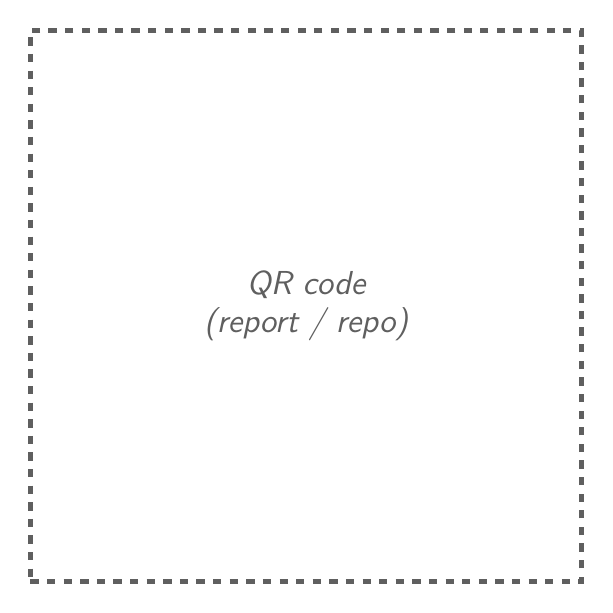
\begin{tikzpicture}
      \node[draw=guidegrey, dashed, line width=2pt, minimum width=7cm,
            minimum height=7cm, text=guidegrey, align=center,
            font=\large\itshape] {QR code\\(report / repo)};
    \end{tikzpicture}%
  }
  \end{center}
  {\small Contact: [email]\\Acknowledgements: instructor, TAs, and the authors
  of the CGHD dataset (CC-BY 4.0).}
}
\end{subcolumns}

\end{columns}
\end{document}
